\documentclass[aspectratio=169]{beamer}
\usepackage[utf8]{inputenc}
\usepackage{booktabs}
\usepackage{tikz}
\usepackage{subcaption}

\usepackage{pgfplots}
\pgfplotsset{compat=1.17}

\usetheme[progressbar=frametitle]{metropolis}
\setbeamertemplate{frame numbering}[fraction]

\graphicspath{{../graphics/}}

% title page
\title{Objectdetectie in sonardata met behulp van semi- en self-supervised learning}
\subtitle{Een verkennend onderzoek naar het toepassen van moderne leertechnieken op onderwaterbeeldvorming}
\author{Yoran Gyselen}
\institute[HOGENT]{Hogeschool Gent}
\date{2024 -- 2025}

\begin{document}
    
    % === Titelpagina ===
    \begin{frame}{}
        \titlepage
    \end{frame}
    
    % === Inhoudstafel ===
    \begin{frame}{Inhoudstafel}
        \tableofcontents
    \end{frame}
    
    % === Introductie ===
    \section{Introductie}
    
    % Sonar
    \begin{frame}{Sonar}
        \begin{itemize}
            \item Sonar = \textbf{Sound Navigation and Ranging}
            \item Gebruikt geluidsgolven om \textbf{onderwaterobjecten en omgevingen te visualiseren}
            \item Types:
            \begin{itemize}
                \item \textbf{Side-scan sonar:} breed zicht, gebruikt voor oppervlaktes
                \item \textbf{Multibeam sonar:} nauwkeurig, gebruikt voor dieptemetingen
                \item \textbf{Synthetic Aperture Sonar (SAS):} evolutie van SSS, veel hogere resolutie
                \item \dots
            \end{itemize}
            \item Output = \textbf{grayscale beelden} met ruis en lage resolutie
            \item Vergelijkbaar met \textbf{``zien van geluid''} onder water
        \end{itemize}
    \end{frame}
    
    \begin{frame}{Voorbeelden van sonarbeelden}
        \begin{figure}
            \centering
            \begin{subfigure}{.5\textwidth}
                \centering
                \captionsetup{justification=centering}
                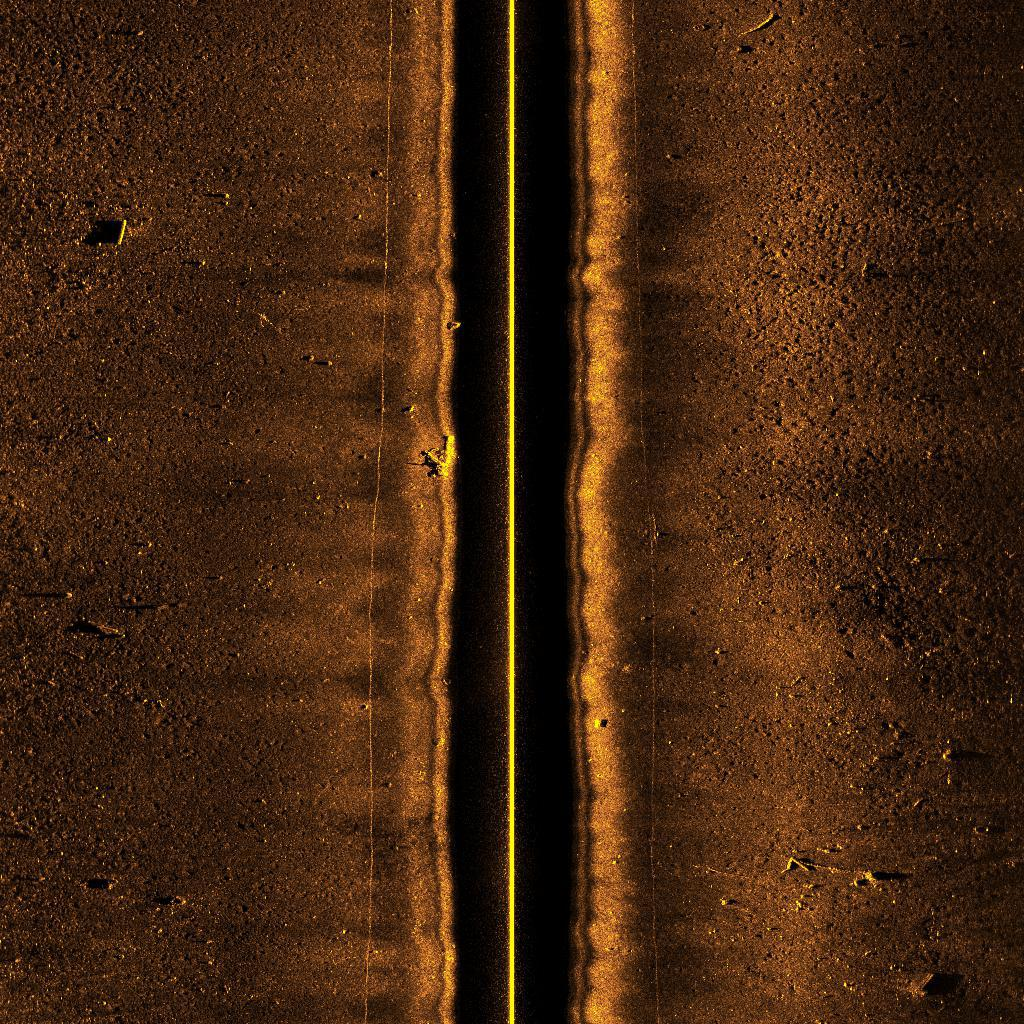
\includegraphics[width=0.9\linewidth]{SSSFMD_example.jpg}
                \caption{Voorbeeld van side-scan sonarbeeld}
            \end{subfigure}%
            \hfill
            \begin{subfigure}{.5\textwidth}
                \centering
                \captionsetup{justification=centering}
                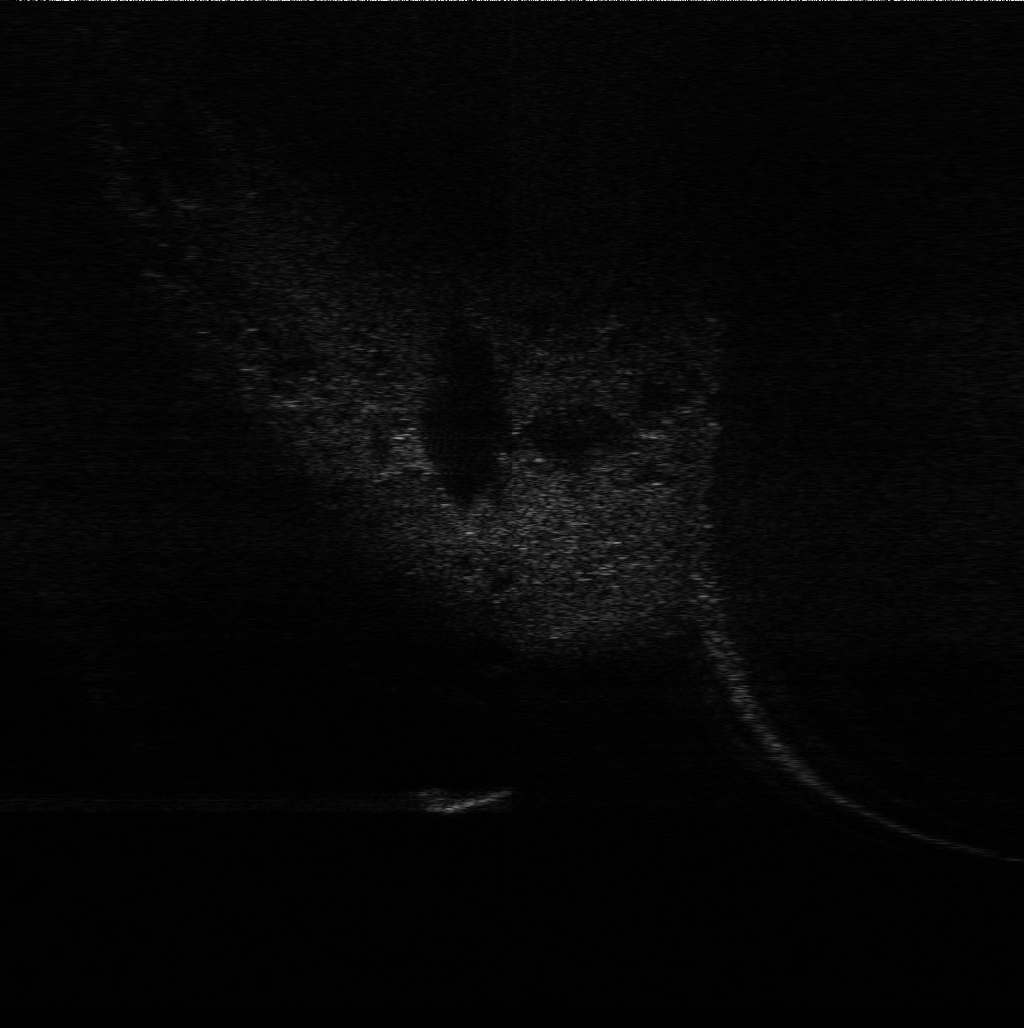
\includegraphics[width=0.9\linewidth]{UATD_example.png}
                \caption{Voorbeeld van multibeam sonarbeeld}
            \end{subfigure}%
        \end{figure}
    \end{frame}
    
    % Belang van objectdetectie op sonarbeelden
    \begin{frame}{Belang van objectdetectie op sonarbeelden}
        \begin{itemize}
            \item \textbf{Mijnenopsporing:} militaire veiligheid in zeeën
            \item \textbf{Archeologisch onderzoek:} wrakken, artefacten vinden
            \item \textbf{Milieustudies:} detecteren van mariene organismen
            \item \textbf{Infrastructuurinspecties:} brugfunderingen, pijpleidingen, zeekabels
        \end{itemize}
        \begin{itemize}
            \item Probleem: veel beelden, \textbf{handmatige analyse is traag en foutgevoelig}
        \end{itemize}
    \end{frame}
    
    \begin{frame}{Voorbeeld van een geannoteerd sonarbeeld}
        \begin{figure}
            \centering
            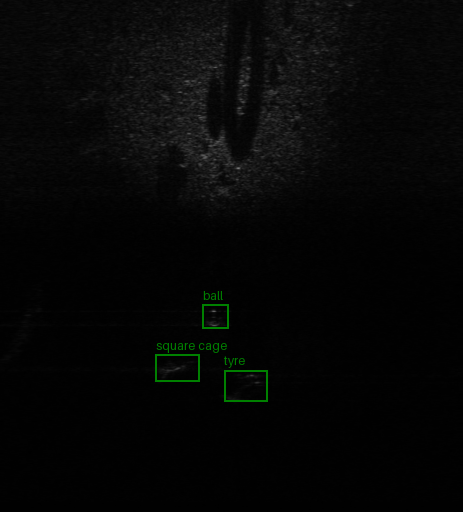
\includegraphics[height=0.9\textheight]{8_gt.png}
        \end{figure}
    \end{frame}
    
    % Motivatie
    \begin{frame}{Motivatie}
        \begin{itemize}
            \item Door stage
            \item Geen ervaring met sonardata
            \item Interesse in toepassingen van objectdetectie
            \item \textit{Real-world} probleem: labelen van sonardata is traag en complex
            \item Toepassen van \textit{cutting-edge} technologieën op bestaand probleem
        \end{itemize}
    \end{frame}
    
    % === Probleemstelling & Onderzoeksvraag ===
    \section{Probleemstelling \& Onderzoeksvraag}
    
    % Problemen bij sonarobjectdetectie
    \begin{frame}{Problemen bij sonarobjectdetectie}
        \begin{itemize}
            \item Sonarbeelden zijn vaag, ruisachtig en moeilijk te interpreteren
            \item Labelen vereist expertise (bv. mijnen herkennen, vorm en context)
            \item Labelproces:
            \begin{itemize}
                \item Tijdrovend
                \item Kostbaar
                \item Niet schaalbaar
            \end{itemize}
        \end{itemize}
    \end{frame}
    
    % Gebrek aan gelabelde data
    \begin{frame}{Gebrek aan gelabelde data}
        \begin{itemize}
            \item \textbf{Geen grote, publieke datasets} zoals bij gewone beelden (COCO, ImageNet)
            \item Vaak \textbf{geclassificeerd} (militair)
            \item \textbf{Niche} $\Rightarrow$ weinig onderzoekers
            \item Veel data nodig voor DL-modellen
        \end{itemize}
    \end{frame}
    
    % Onderzoeksvraag
    \begin{frame}{Onderzoeksvraag}
        \textbf{Doel:} optimaliseren van workflow waarbij (heel) veel gelabelde data nodig is
        
        \vspace{\baselineskip}
        
        \begin{quote}
            \textbf{Onderzoeksvraag:} \\
            Kunnen semi- en self-supervised leermethoden het labelproces versnellen zonder een significant verlies in nauwkeurigheid?
        \end{quote}
        
        \begin{itemize}
            \item Prestatie van deze methodes t.o.v. volledig supervised modellen?
            \item Minimale hoeveelheid gelabelde data?
            \item Best werkende techniek(en)?
        \end{itemize}
    \end{frame}
    
    % === Achtergrond & Theoretisch kader ===
    \section{Achtergrond \& Theoretisch kader}
    
    % Objectdetectie
    \begin{frame}{Objectdetectie}
        \textbf{Doel:} lokaliseren \& classificeren van objecten in afbeeldingen
        
        \vspace{\baselineskip}
        
        Twee grote types modellen:
        
        \begin{itemize}
            \item \textbf{Single-shot:} heel snel, minder precies \\ Bv. YOLO (You Only Look Once) \& SSD (Single Shot MultiBox Detector)
            \item \textbf{Two-stage:} trager, maar nauwkeuriger \\ Bv. Faster R-CNN
        \end{itemize}
    \end{frame}
    
    \begin{frame}{SSD- vs. YOLO-architectuur}
        \begin{figure}
            \centering
            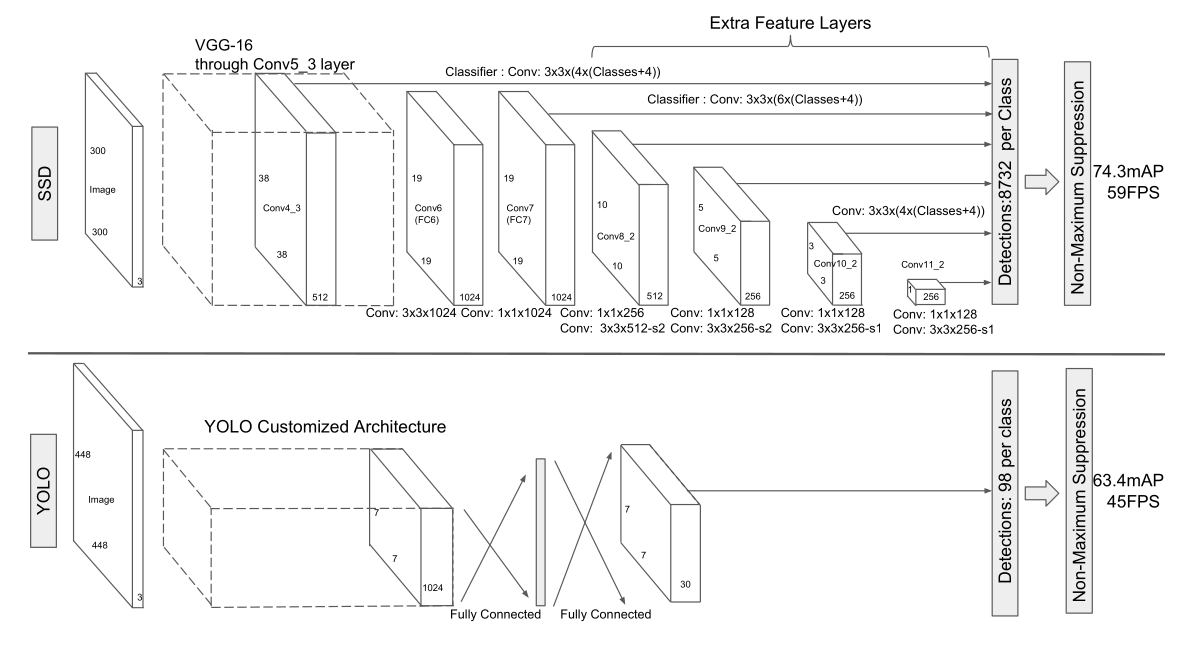
\includegraphics[height=0.9\textheight]{ssd_architecture.png}
        \end{figure}
    \end{frame}
    
    \begin{frame}{Faster R-CNN-architectuur}
        \begin{figure}
            \centering
            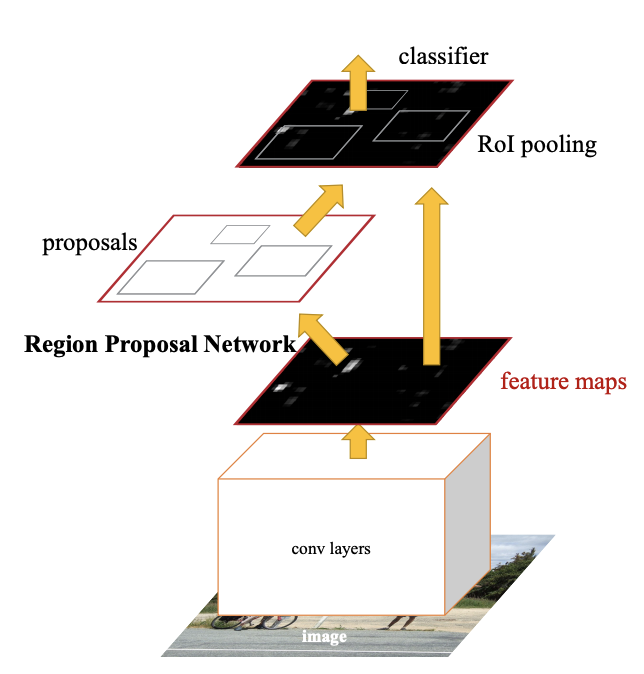
\includegraphics[height=0.9\textheight]{faster_rcnn_architecture.png}
        \end{figure}
    \end{frame}
    
    % Supervised learning
    \begin{frame}{Supervised learning}
        \begin{itemize}
            \item Leert op basis van \textbf{gelabelde data}
            \item Nodig: afbeeldingen + bounding boxes (bv. mijnen)
            \item \textbf{Zeer accuraat} bij veel data
            \item \textbf{Probleem:} labelen is duur \& tijdrovend
        \end{itemize}
    \end{frame}
    
    % Semi-supervised learning
    \begin{frame}{Semi-supervised learning}
        \textbf{Semi-supervised learning (SSL)}
        \begin{itemize}
            \item Combineert \textbf{kleine hoeveelheid gelabelde data} met veel ongelabelde data
            \item Typische technieken:
            \begin{itemize}
                \item \textbf{Pseudo-labeling:} model genereert labels voor onbekende data
                \item \textbf{Consistency regularization:} model leert robuust te blijven bij kleine veranderingen in input (bv. rotatie, ruis)
            \end{itemize}
            \item \textbf{Data-augmentatie} speelt een centrale rol
        \end{itemize}
    \end{frame}
    
    % Self-supervised learning
    \begin{frame}{Self-supervised learning}
        \textbf{Self-supervised learning (Self-SL)}
        \begin{itemize}
            \item \textbf{Geen gelabelde data nodig} tijdens pre-training
            \item Model leert door \textbf{pretext-taken}: kunstmatige taken die de structuur van data onthullen
            \item Typische technieken:
            \begin{itemize}
                \item \textbf{Contrastive learning:} vergelijk gelijkaardige vs. niet-gelijkaardige beelden
                \item \textbf{Predictieve taken:} bv. voorspellen van ontbrekende delen of transformaties
                \item \textbf{Representation learning:} model leert algemene kenmerken extraheren
            \end{itemize}
        \end{itemize}
    \end{frame}
    
    % Voordelen bij sonardata
    \begin{frame}{Voordelen bij sonardata}
        \begin{itemize}
            \item Sonardata is:
            \begin{itemize}
                \item Moeilijk te interpreteren
                \item Schaars in gelabelde vorm
            \end{itemize}
            \item SSL \& Self-SL laten modellen leren uit veel \textbf{ongelabelde data}
        \end{itemize}
        \begin{enumerate}[$\Rightarrow$]
            \item Grote tijds- en kostbesparing
            \item Vergelijkbare nauwkeurigheid bij weinig gelabelde data
        \end{enumerate}
    \end{frame}
    
    % === Methodologie & Experimentele opzet ===
    \section{Methodologie \& Experimentele opzet}
    
    % Dataset & Data-opzet
    \begin{frame}{Dataset \& Data-opzet}
        \textbf{Dataset:}
        \begin{itemize}
            \item Publieke sonarbeeld-dataset: \textbf{7600 afbeeldingen}
            \item Beelden bevatten \textbf{onderwaterobjecten} zoals mijnen of wrakken
            \item Enkel subset van beelden handmatig gelabeld
        \end{itemize}
        \textbf{Dataverdeling:} \\
        Getest met verschillende labelpercentages:
        \begin{itemize}
            \item 1\%, 5\%, 10\%, 50\%, 100\% \textbf{gelabeld}
            \item Resterende data als \textbf{ongelabelde input}
        \end{itemize}
    \end{frame}
    
    % Vergelijking van 3 leertechnieken
    \begin{frame}{Vergelijking van leermethoden}
        \centering
        \begin{tabular}{lll}
            \toprule
            \textbf{Type} & \textbf{Methode} & \textbf{Doel} \\
            \midrule
            Supervised      & Faster R-CNN       & Alleen gelabelde data \\
            Semi-supervised & + FixMatch         & Weinig labels + pseudo-labels \\
            Self-supervised & + BYOL (pre-train) & Pre-training zonder labels, daarna fine-tunen \\
            \bottomrule
        \end{tabular}
    \end{frame}
    
    % Trainen & Evalueren
    \begin{frame}{Trainen \& Evalueren}
        \textbf{Training details:}
        \begin{itemize}
            \item Deep learning framework: PyTorch
            \item Veel gebruik gemaakt van TorchVision
            \item Gebruik van GPU (NVIDIA RTX A5000)
            \item Optimalisatietechnieken:
            \begin{itemize}
                \item Early stopping
                \item Mixed precision training
                \item Lagen bevriezen
                \item Linear warm-up
                \item \dots
            \end{itemize}
        \end{itemize}
        \textbf{Evaluatiemethode:}
        \begin{itemize}
            \item Prestatie gemeten met mAP-score (mean Average Precision)
            \item Gebruik van loss-functie voor evaluatie
        \end{itemize}
    \end{frame}
    
    % Doel van vergelijking
    \begin{frame}{Doel van vergelijking}
        \begin{itemize}
            \item Hoe robuust zijn modellen bij weinig gelabelde data?
            \item Test per model bij 1\%, 5\%, 10\%, 50\%, 100\% gelabeld
        \end{itemize}
        \begin{enumerate}[$\Rightarrow$]
            \item Directe vergelijking van prestaties
            \item Welke strategie werkt het best met zo min mogelijk manueel werk?
        \end{enumerate}
    \end{frame}
    
    % === Resultaten ===
    \section{Resultaten}
    
    % mAP-score (mean Average Precision)
    \begin{frame}{mAP-score (mean Average Precision)}
        \textbf{mAP} meet hoe goed het model objecten:
        \begin{itemize}
            \item Correct lokaliseert (bounding boxes)
            \item Correct classificeert
        \end{itemize}
        \textbf{Belangrijk:}
        \begin{itemize}
            \item Waarde tussen 0 en 1
            \item Hoe hoger de mAP, hoe beter
            \item mAP combineert \textit{precision} en \textit{recall} over verschillende klassen en drempels
        \end{itemize}
    \end{frame}
    
    % Kwantitatief overzicht van de supervised resultaten
    \begin{frame}{Kwantitatief overzicht van de supervised resultaten}
        \centering
        \begin{tikzpicture}
            \begin{axis}[
                ybar,
                width=\textwidth,
                height=\textheight,
                symbolic x coords={100\%, 50\%, 10\%, 5\%, 1\%},
                xtick=data,
                ymin=0,
                bar width=15pt,
                xlabel={Verschillende data-splits},
                ylabel={mAP-score},
                nodes near coords,
                ]
                \addplot coordinates {(100\%,0.7717) (50\%,0.7847) (10\%,0.6152) (5\%,0.5298) (1\%,0.2799)};
            \end{axis}
        \end{tikzpicture}
    \end{frame}
    
    % Kwalitatief overzicht van de supervised resultaten
    \begin{frame}{Kwalitatief overzicht van de supervised resultaten}
        \begin{figure}
            \centering
            \begin{subfigure}{.15\textwidth}
                \centering
                \captionsetup{justification=centering}
                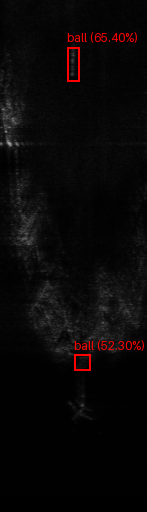
\includegraphics[width=0.9\linewidth]{251_faster_rcnn_1pct.png}
                \caption[Voorspelling Faster R-CNN 1\%]{1\%}
            \end{subfigure}%
            \hfill
            \begin{subfigure}{.15\textwidth}
                \centering
                \captionsetup{justification=centering}
                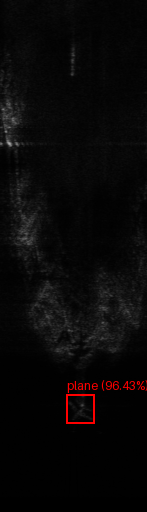
\includegraphics[width=0.9\linewidth]{251_faster_rcnn_5pct.png}
                \caption[Voorspelling Faster R-CNN 5\%]{5\%}
            \end{subfigure}%
            \hfill
            \begin{subfigure}{.15\textwidth}
                \centering
                \captionsetup{justification=centering}
                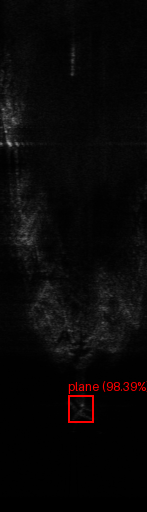
\includegraphics[width=0.9\linewidth]{251_faster_rcnn_10pct.png}
                \caption[Voorspelling Faster R-CNN 5\%]{5\%}
            \end{subfigure}%
            \hfill
            \begin{subfigure}{.15\textwidth}
                \centering
                \captionsetup{justification=centering}
                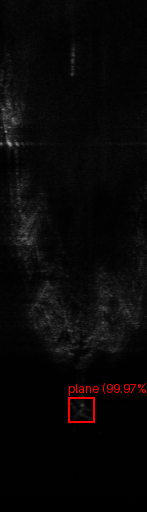
\includegraphics[width=0.9\linewidth]{251_faster_rcnn_50pct.png}
                \caption[Voorspelling Faster R-CNN 50\%]{50\%}
            \end{subfigure}%
            \hfill
            \begin{subfigure}{.15\textwidth}
                \centering
                \captionsetup{justification=centering}
                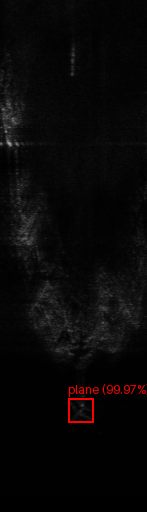
\includegraphics[width=0.9\linewidth]{251_faster_rcnn_100pct.png}
                \caption[Voorspelling Faster R-CNN 100\%]{100\%}
            \end{subfigure}%
        \end{figure}
    \end{frame}
    
    % Kwantitatief overzicht van de semi- en self-supervised resultaten
    \begin{frame}{Kwantitatief overzicht van de semi- en self-supervised resultaten}
        \centering
        \begin{tikzpicture}
            \begin{axis}[
                ybar,
                bar width=15pt,
                width=\textwidth,
                height=0.9\textheight,
                enlargelimits=0.5,
                ybar=10pt,
                legend style={at={(0.5,-0.15)}, anchor=north,legend columns=-1},
                xlabel={Verschillende data-splits},
                ylabel={mAP-score},
                ymax=0.7,
                symbolic x coords={10\%, 5\%},
                xtick=data,
                nodes near coords,
                nodes near coords align={vertical},
                ]
                \addplot coordinates {(10\%,0.6152) (5\%,0.5298)};
                \addplot coordinates {(10\%,0.6828) (5\%,0.6649)};
                \addplot coordinates {(10\%,0.7230) (5\%,0.6452)};
                \legend{Faster R-CNN baseline, FixMatch, BYOL}
            \end{axis}
        \end{tikzpicture}
    \end{frame}
    
    % Kwalitatief overzicht van de semi- en self-supervised resultaten
    \begin{frame}{Kwalitatief overzicht van de semi- en self-supervised resultaten}
        \begin{figure}
            \centering
            \begin{subfigure}{.2\textwidth}
                \centering
                \captionsetup{justification=centering}
                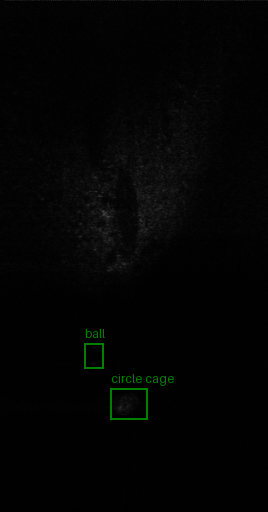
\includegraphics[width=0.9\linewidth]{1_gt.png}
                \caption{Ground truth}
            \end{subfigure}%
            \begin{subfigure}{.2\textwidth}
                \centering
                \captionsetup{justification=centering}
                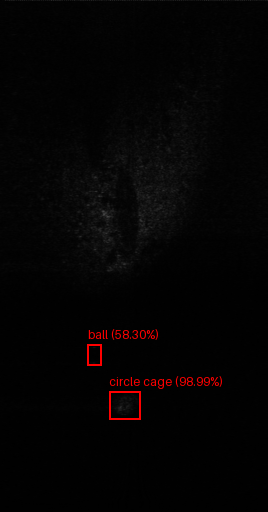
\includegraphics[width=0.9\linewidth]{1_fixmatch_10pct.png}
                \caption{FixMatch 10\%}
            \end{subfigure}%
            \begin{subfigure}{.2\textwidth}
                \centering
                \captionsetup{justification=centering}
                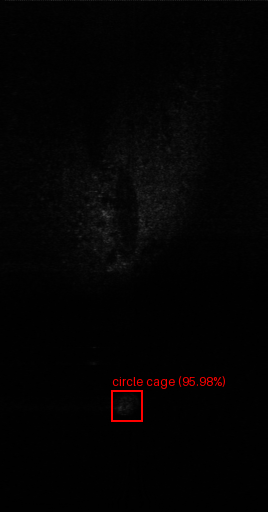
\includegraphics[width=0.9\linewidth]{1_fixmatch_5pct.png}
                \caption{FixMatch 5\%}
            \end{subfigure}%
            \begin{subfigure}{.2\textwidth}
                \centering
                \captionsetup{justification=centering}
                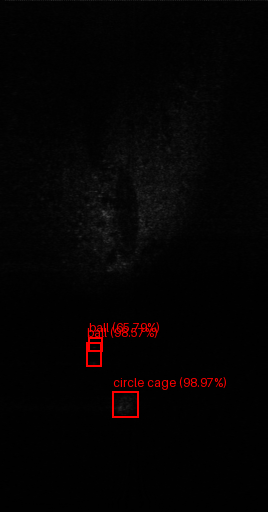
\includegraphics[width=0.9\linewidth]{1_faster_rcnn_10_byol.png}
                \caption{BYOL 10\%}
            \end{subfigure}%
            \begin{subfigure}{.2\textwidth}
                \centering
                \captionsetup{justification=centering}
                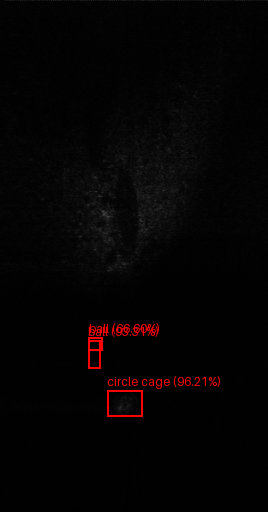
\includegraphics[width=0.9\linewidth]{1_faster_rcnn_5_byol.png}
                \caption{BYOL 5\%}
            \end{subfigure}%
        \end{figure}
    \end{frame}
    
    % === Conclusie & Reflectie ===
    \section{Conclusie \& Reflectie}
    
    % Conclusies uit de resultaten
    \begin{frame}{Conclusies uit de resultaten}
        \begin{itemize}
            \item \textbf{Supervised learning (Faster R-CNN):}
            \begin{itemize}
                \item Presteert duidelijk minder met weinig data
            \end{itemize}
            \item \textbf{Semi-supervised learning (FixMatch):}
            \begin{itemize}
                \item Presteert beter dan supervised bij weinig data (5-10\%)
                \item Biedt een sterke balans tussen eenvoud en prestatie
            \end{itemize}
            \item \textbf{Self-supervised learning (BYOL):}
            \begin{itemize}
                \item Beste prestaties bij 10\% gelabelde data
                \item Groot potentieel voor moeilijk labelbare domeinen zoals sonar
            \end{itemize}
        \end{itemize}
    \end{frame}
    
    % Reflectie op het onderzoek
    \begin{frame}{Reflectie op het onderzoek}
        \textbf{Sterke punten:} \\
        \begin{itemize}
            \item Geschikte keuze van modellen \& dataset
            \item Focus op een praktisch probleem uit de industrie
            \item Heldere vergelijkingsstructuur tussen drie leermethoden
        \end{itemize}
        \textbf{Beperkingen:} \\
        \begin{itemize}
            \item Moeilijkheden bij implementatie \& optimalisatie van modellen
            \item Grote computationele requirements
            \item Slechts beperkte optimalisatie
        \end{itemize}
    \end{frame}
    
    % Toekomstig onderzoek
    \begin{frame}{Toekomstig onderzoek}
        \begin{itemize}
            \item Andere pre-trainingstechnieken (SimCLR, MoCo, DINO, \dots)
            \item Andere backbones (ResNet, Swin Transformer, ConvNeXt, \dots)
            \item Geschiktere SSL-technieken (FlexMatch, SoftMatch, UDA, \dots)
            \item Transfer learning
            \item Combinatie van technieken: bv. BYOL + FixMatch
            \item Actieve leerstrategieën: slim kiezen welke samples gelabeld worden
            \item Foutenanalyse \& XAI
            \item \dots
        \end{itemize}
    \end{frame}
    
    % === Vragen ===
    \section{Vragen}
    
    % === Titelpagina ===
    \begin{frame}{}
        \titlepage
    \end{frame}
\end{document}